\chapter{Structure of Cell Membrane}

\begin{introduction}
	\item 
\end{introduction}

\begin{emptytcb*}{functions of cell membranes}{}
	
	\begin{itemize}
		\item
		compartmentalization
		\item
		selective permeable
		\item
		communication, signal transduction
		\item
		organize activities, energy production
	\end{itemize}
\end{emptytcb*}


\hypertarget{lipids}{%
	\section{Lipids}\label{lipids}}

\hypertarget{types}{%
	\subsection{types}\label{types}}

\begin{itemize}
	\item
	glycerophospholipids
	\item
	sphingolipids
	\item
	cholesterol
\end{itemize}
\hypertarget{features}{%
	\subsection{features}\label{features}}

\begin{itemize}
	\item
	\textbf{amphiphilic}
	\item
	different content in different species or organs
\end{itemize}

\begin{figure}
	\centering
	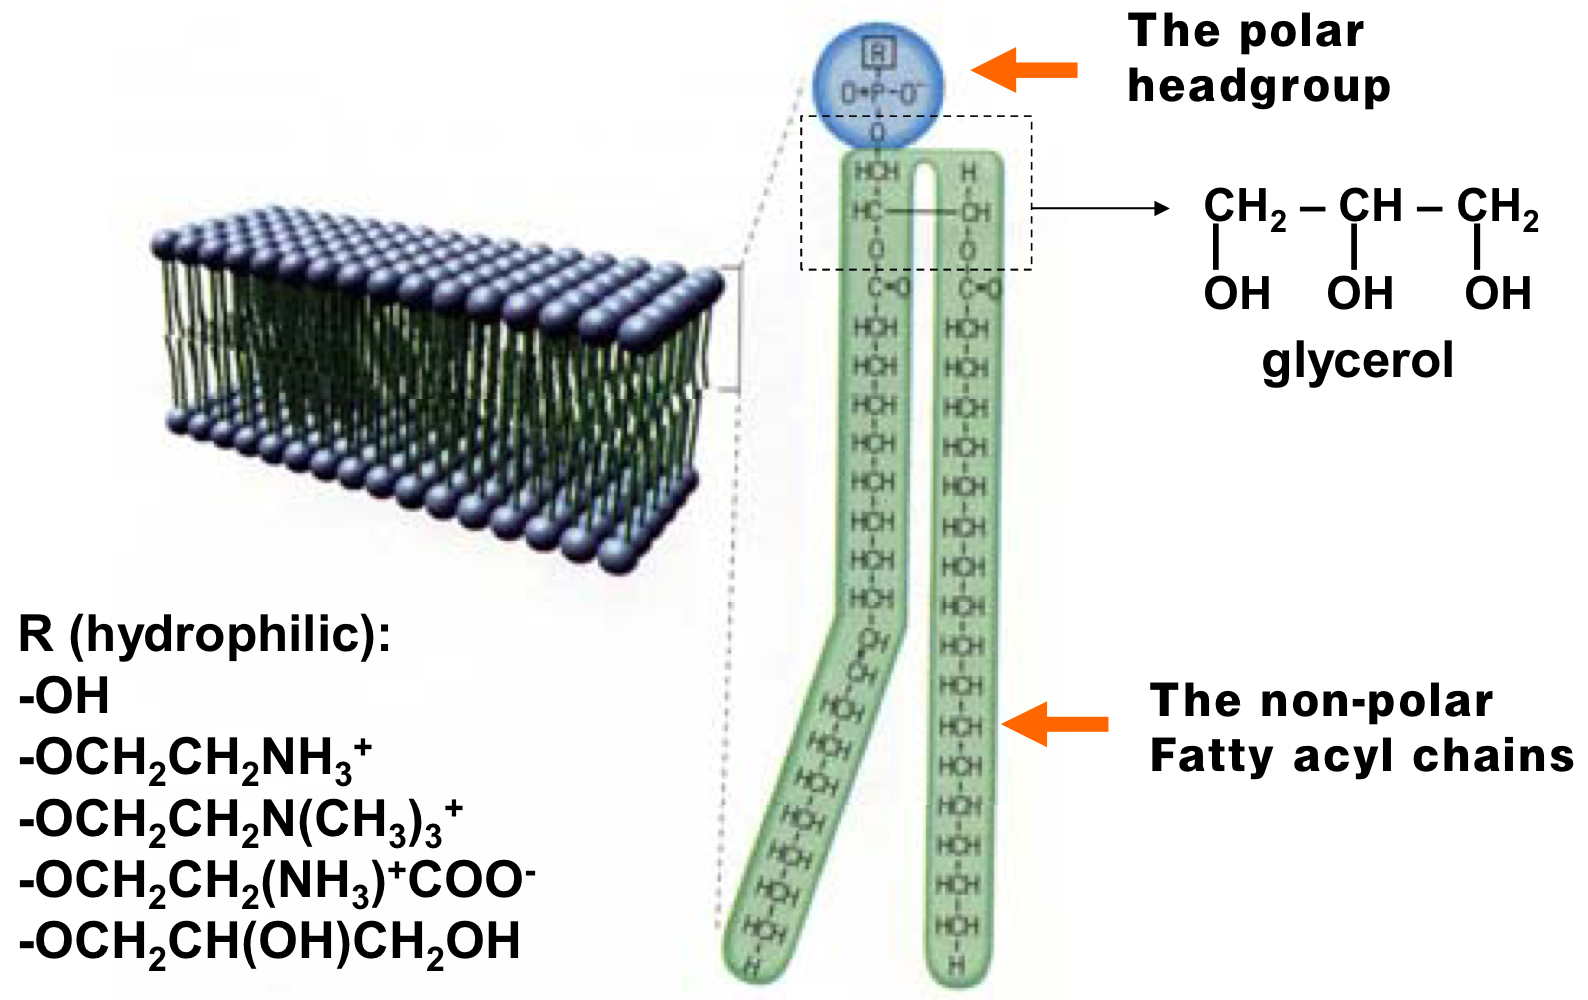
\includegraphics[width=0.5\linewidth]{E:/undergraduate_study/study/abroad study/2021 NUS/study/LSM3243/notes/3_1.png}
%	\caption{3\_1}
\end{figure}

\hypertarget{lipids-on-the-membrane}{%
	\section{lipids on the membrane}\label{lipids-on-the-membrane}}

\begin{enumerate}
	\def\labelenumi{\arabic{enumi}.}
	\item
	\textbf{assymetric} distribution (in two layers)
	
	\begin{itemize}
		\item
		negative charged phospholipids tend to point at cytosol while the
		neutral ones point at extracellular space
		
		when cell undergoes apoptosis, POPS goes to the outer membrane because entropy increases.
	\end{itemize}
	\item
	\textbf{random} distribution (in the same layer)
	
	\begin{itemize}
		\item
		lipids are randomly distributed, and swim.. (bulk phase)
		
		\begin{itemize}
			\item
			\underline{vdW forces are not strong enough to hold lipids together}
			\item
			hydrophobic effect drives the lipid to assemble, so there must be
			water
		\end{itemize}
	\end{itemize}
\end{enumerate}

\begin{figure}
	\centering
	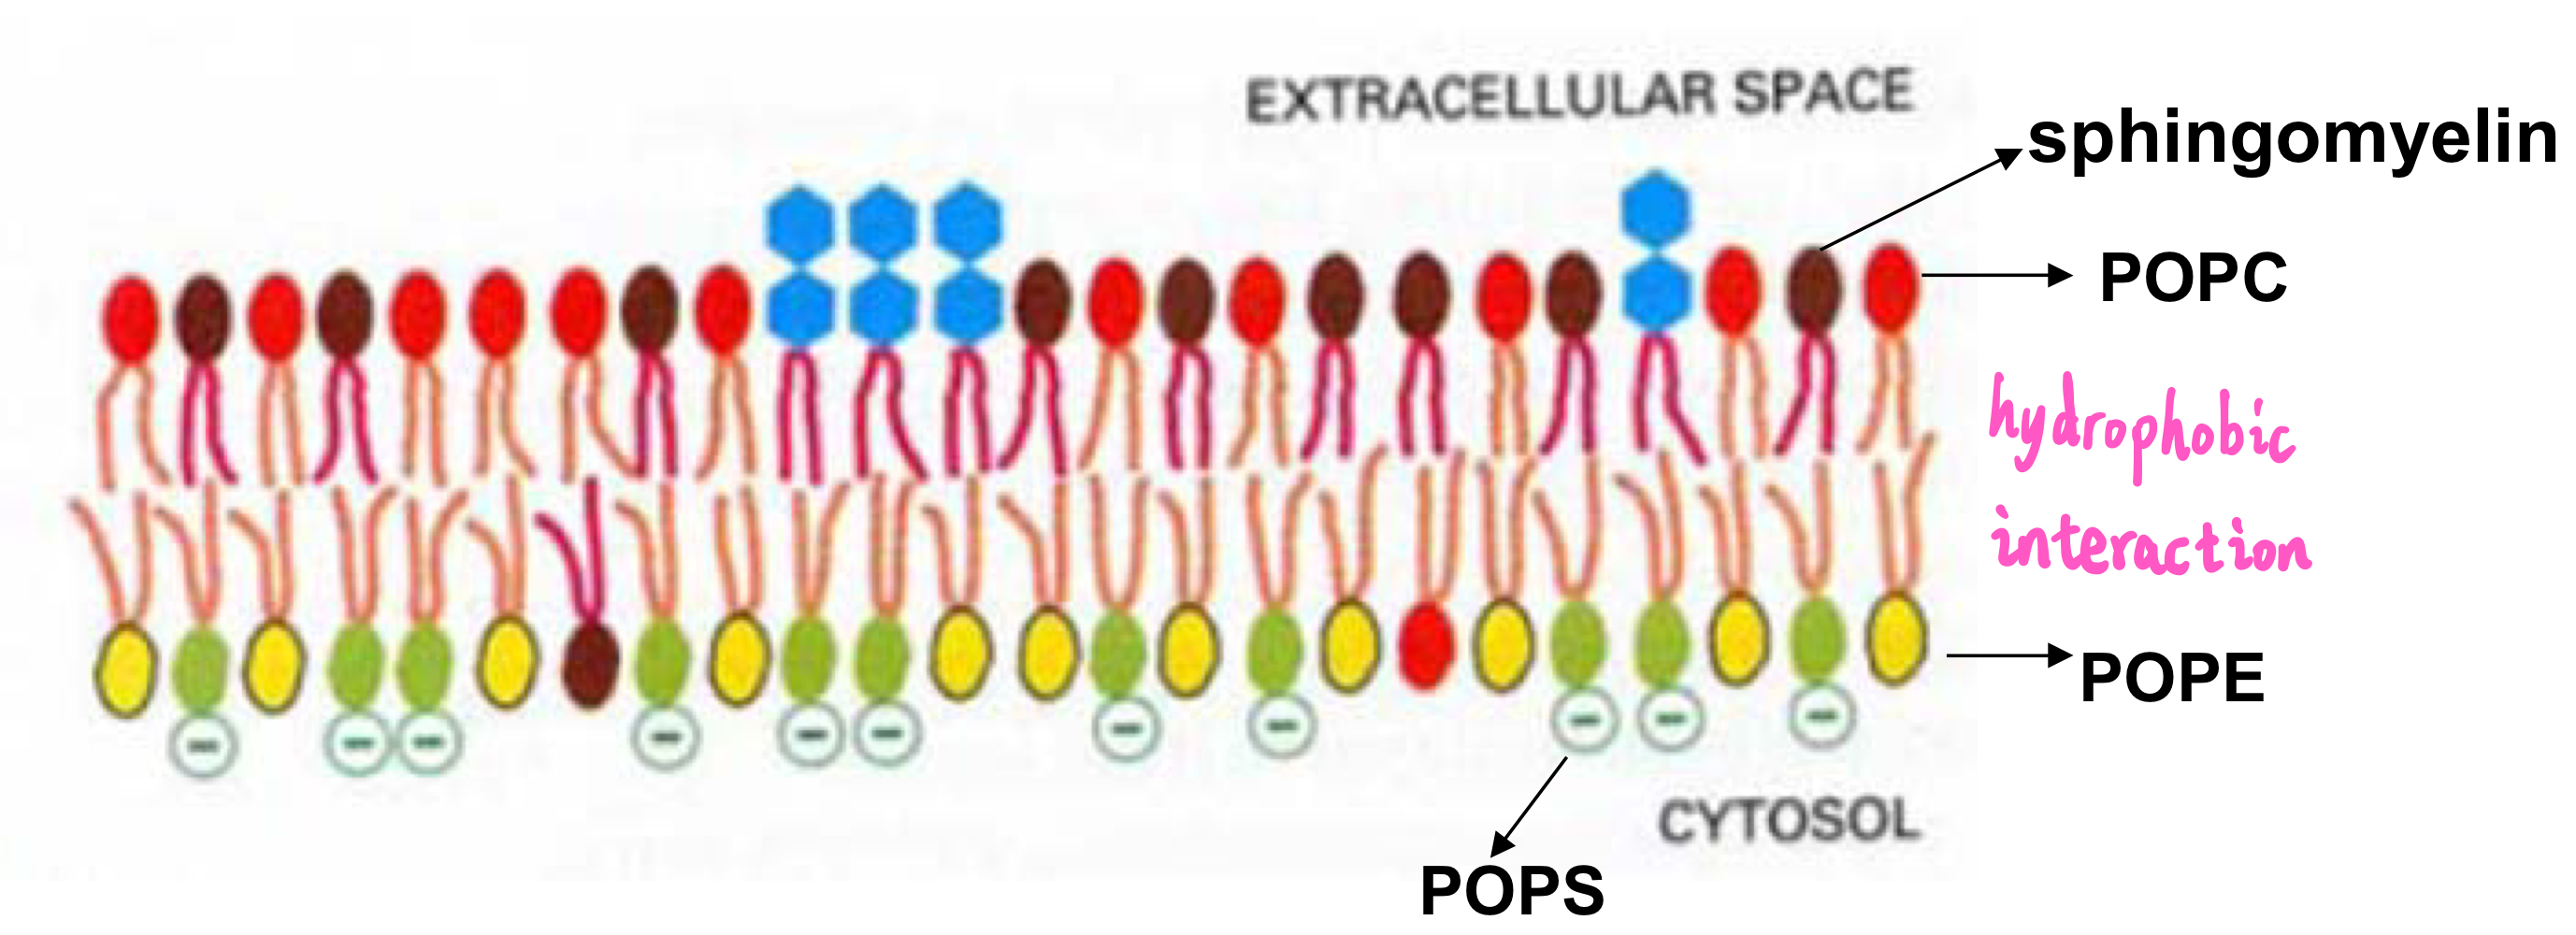
\includegraphics[width=0.7\linewidth]{E:/undergraduate_study/study/abroad study/2021 NUS/study/LSM3243/notes/3_2.png}
%	\caption{3\_2}
\end{figure}

\hypertarget{lipid-rafts}{%
	\section{lipid rafts}\label{lipid-rafts}}

\begin{itemize}
	\item
	sphingolipids have longer and straighter fatty acids
	
	thus have bigger vdW forces to hold themselves together (transiently)
	
	\begin{itemize}
		\item
		glycerophospholipids: about 13?
	\end{itemize}
	\item
	cholesterol can hold more lipid molecules
	
	\begin{itemize}
		\item
		it's also very "hydrophobic"
		\item
		it interacts with fatty acids in both sides of the plane, and has
		bigger surface area.
		\item
		its ring is a rigid structure that makes lipid rafts stable.
	\end{itemize}
\end{itemize}

\begin{figure}
	\centering
	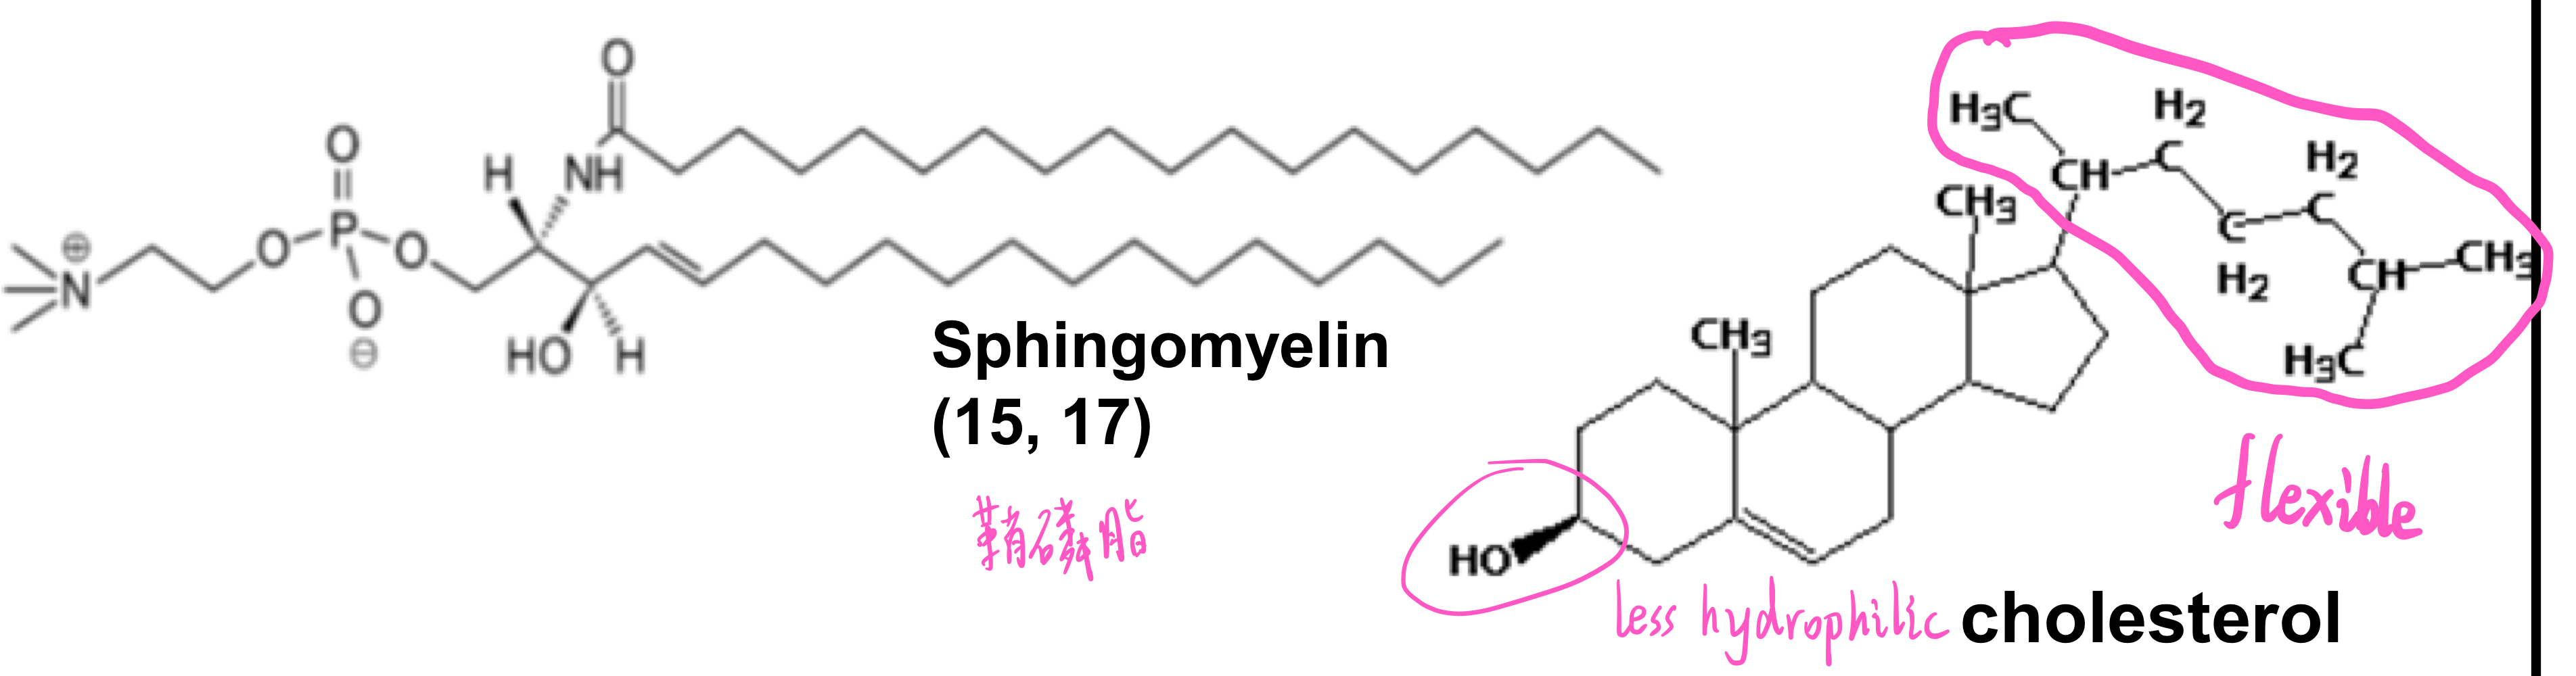
\includegraphics[width=0.8\linewidth]{3_3.png}
%	\caption{}
\end{figure}

They assembly into lipid rafts, which

\begin{itemize}
	\item
	are thicker (longer) than other parts of the membrane;
	\item
	are more resistant to detergents
	\item
	accommodate and gather proteins for specific functions like singaling
\end{itemize}

\begin{figure}
	\centering
	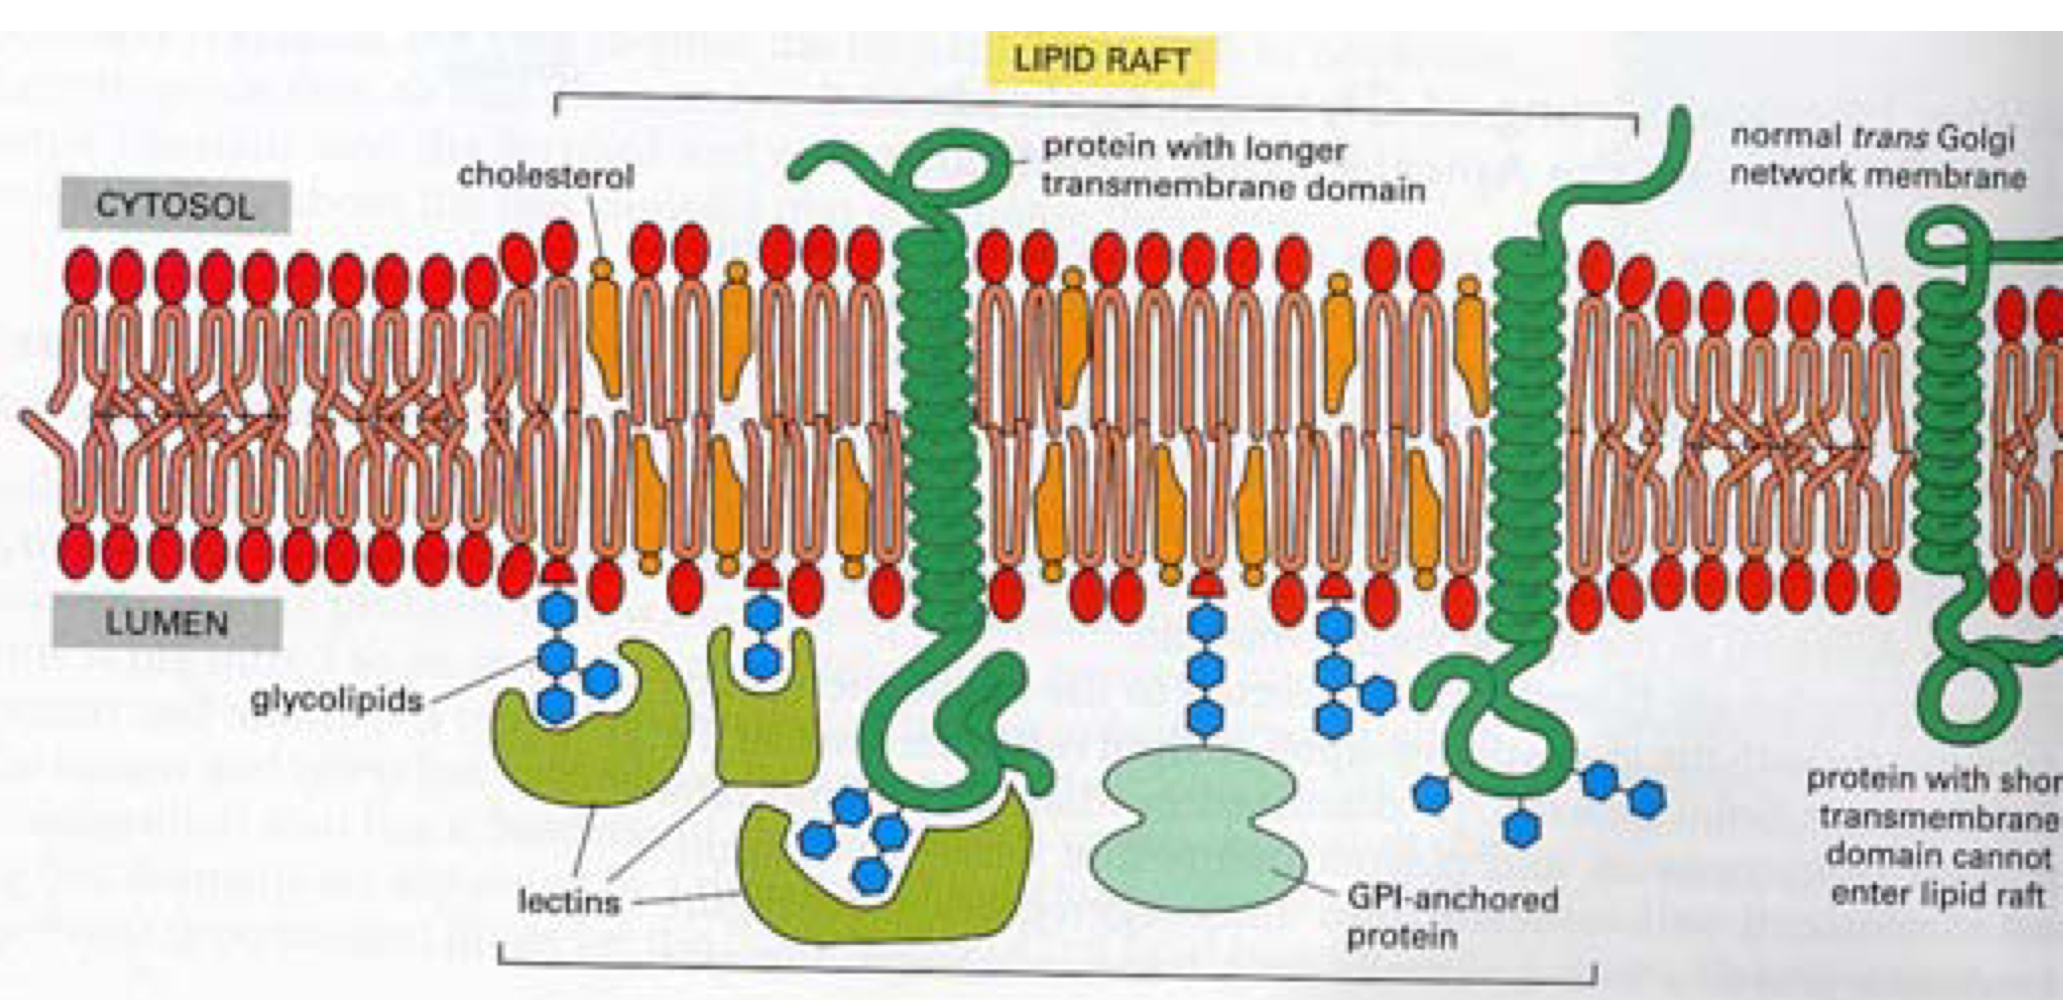
\includegraphics[width=0.9\linewidth]{3_4.png}
%	\caption{}
\end{figure}

\hypertarget{proteins}{%
	\section{proteins}\label{proteins}}

ratio \(\uparrow\), function \(\uparrow\)

\begin{emptytcb*}{References}{}
\href{https://en.wikipedia.org/wiki/Membrane_protein}{see figures}

\href{https://www.expasy.org/resources/protscale}{hydrophobicity plot tool}

\end{emptytcb*}

Types of membrane proteins:

\begin{itemize}
	\item
	integral
	
	\begin{itemize}
		\item
		one or multiple \textbf{transmembrane} segments
		\item
		\(\alpha\) helix or \(\beta\) barrel
		\item hydrophobic R chains point outwards (maybe hydrophilic inwards)
		\item
		some are not trans-membrane
	\end{itemize}
	\item
	peripheral
	
	\begin{itemize}
		\item
		no covalent bonds, only \textbf{non-covalent} bonds
		
		\begin{itemize}
			\item
			electrostatically: with polar head
			\item
			terminal hydrophobic group: with bilayer core
			\item
			or bound to an integral protein
		\end{itemize}
		
		either outside and inside the membrane
	\end{itemize}
	\item
	anchored
	
	\begin{itemize}
		\item
		\textbf{covalently} bond to the lipids
		\item
		GPI-anchored proteins (G: glycosylphosphatidylinositol-linked)
		
		\begin{itemize}
			\item
			protein--phosphoethanolamine-\/-\/-tetrasaccharide-\/-\/-inositol-\/-\/-
			
			\begin{itemize}
				\item
				where lipase C functions
			\end{itemize}
			\item
			phosphate-\/-\/-diacylglycerol, which is a part of bilayer
		\end{itemize}
		\item
		function: enzyme, antigen, adhesion
	\end{itemize}
\end{itemize}

\begin{figure}
	\centering
	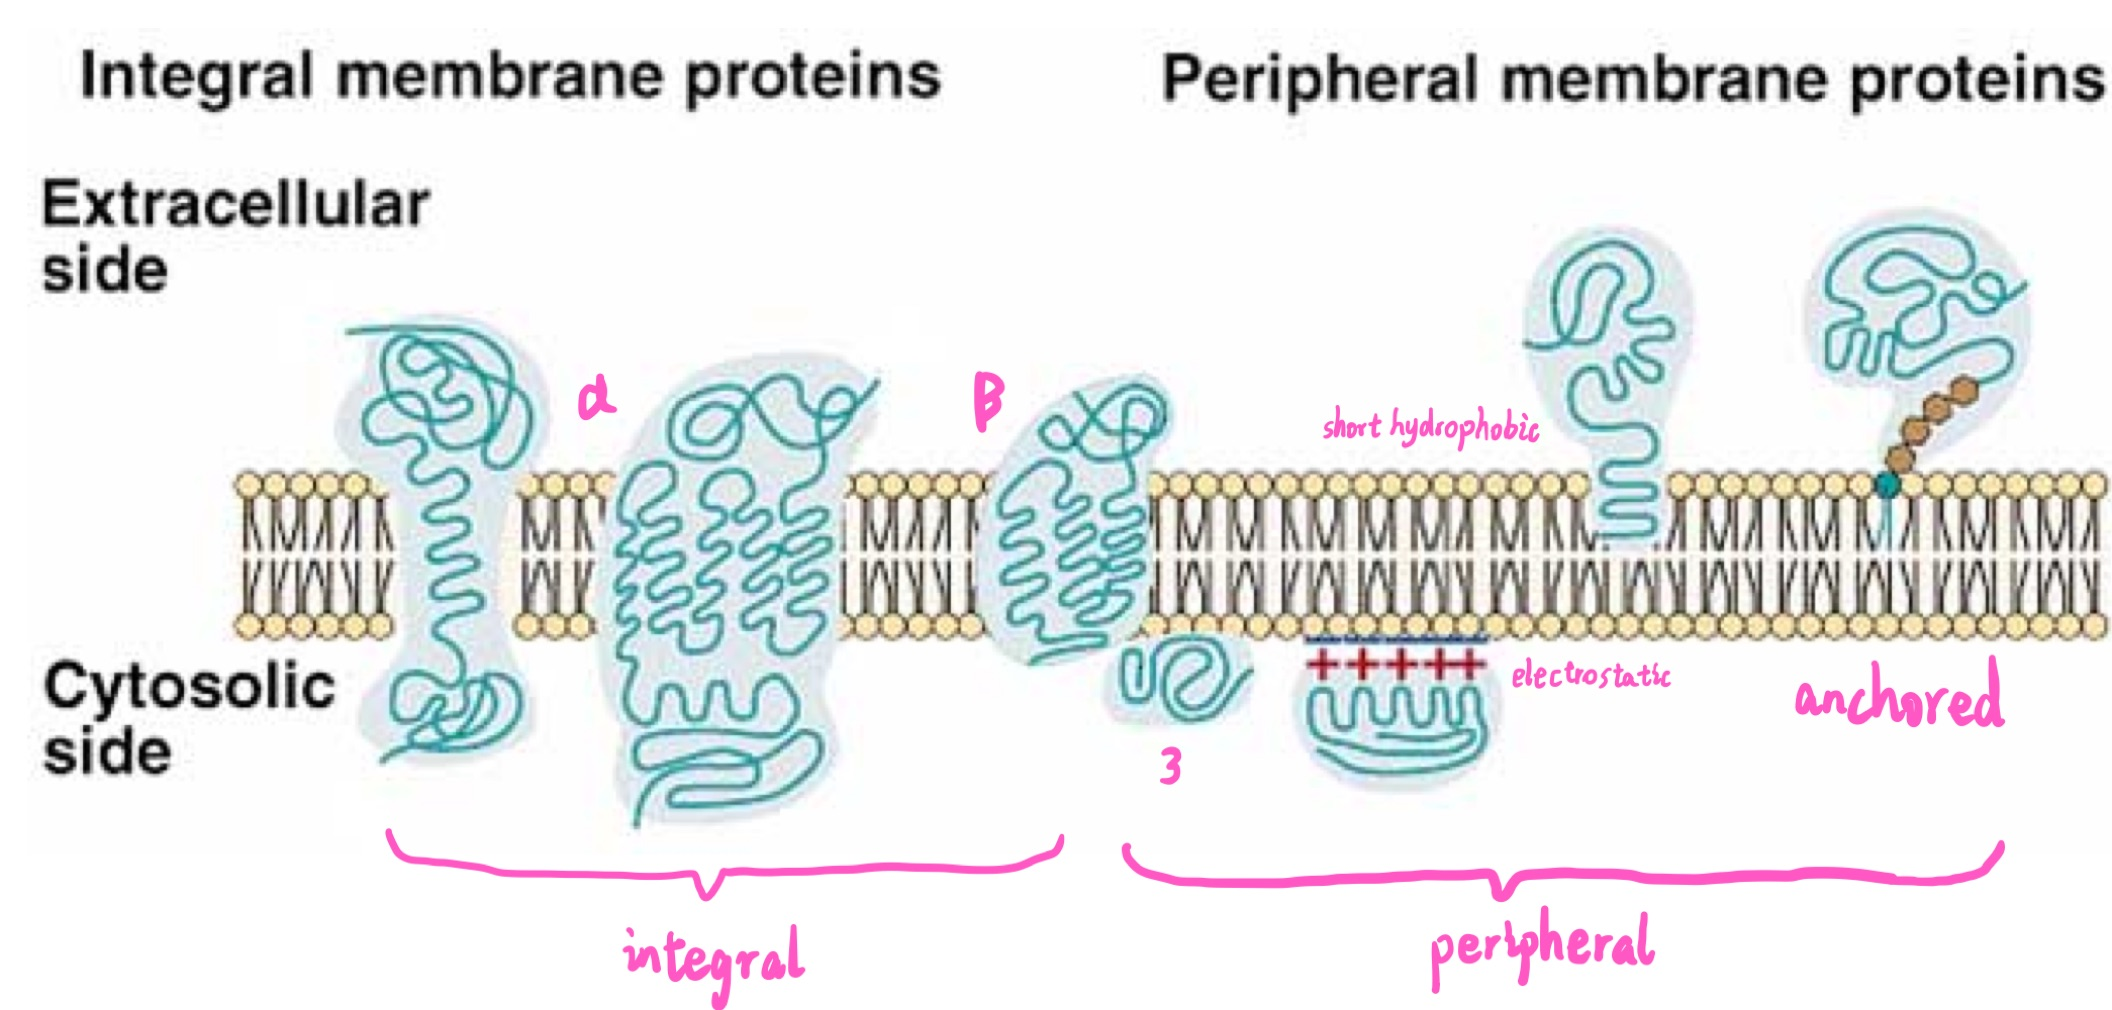
\includegraphics{E:/undergraduate_study/study/abroad study/2021 NUS/study/LSM3243/notes/3_5.jpg}
	\caption{}
\end{figure}

\hypertarget{micelles}{%
	\section{micelles}\label{micelles}}

\url{https://en.wikibooks.org/wiki/Structural_Biochemistry/Lipids/Micelles}

\begin{itemize}
	\item
	as the concentration of detergent/lipid molecules rises (over Critical
	Micelle Concentration, CMC), they are no more a layer on the surface,
	but forms micelles (胶束).
	\item
	structure
	
	\begin{itemize}
		\item
		SDS can be seen as a cone (圆锥) model
		
		which is due to electrostatic repulsion on the heads 
		
		\begin{itemize}
			\item
			driven by hydrophobic interaction, they form a sphere
			\item
			when concentration get higher, the sphere get bigger and water
			enter inside, thus hydrophobic interaction is disrupted.
		\end{itemize}
		\item
		DPC is a zwitterion but has to be parallel (replusion direction) to
		avoid contacting hydrophobic groups.
		\item
		triglyceride may form a cylinder, which favours the formation of
		bilayer.
	\end{itemize}
\end{itemize}

\begin{figure}
	\centering
	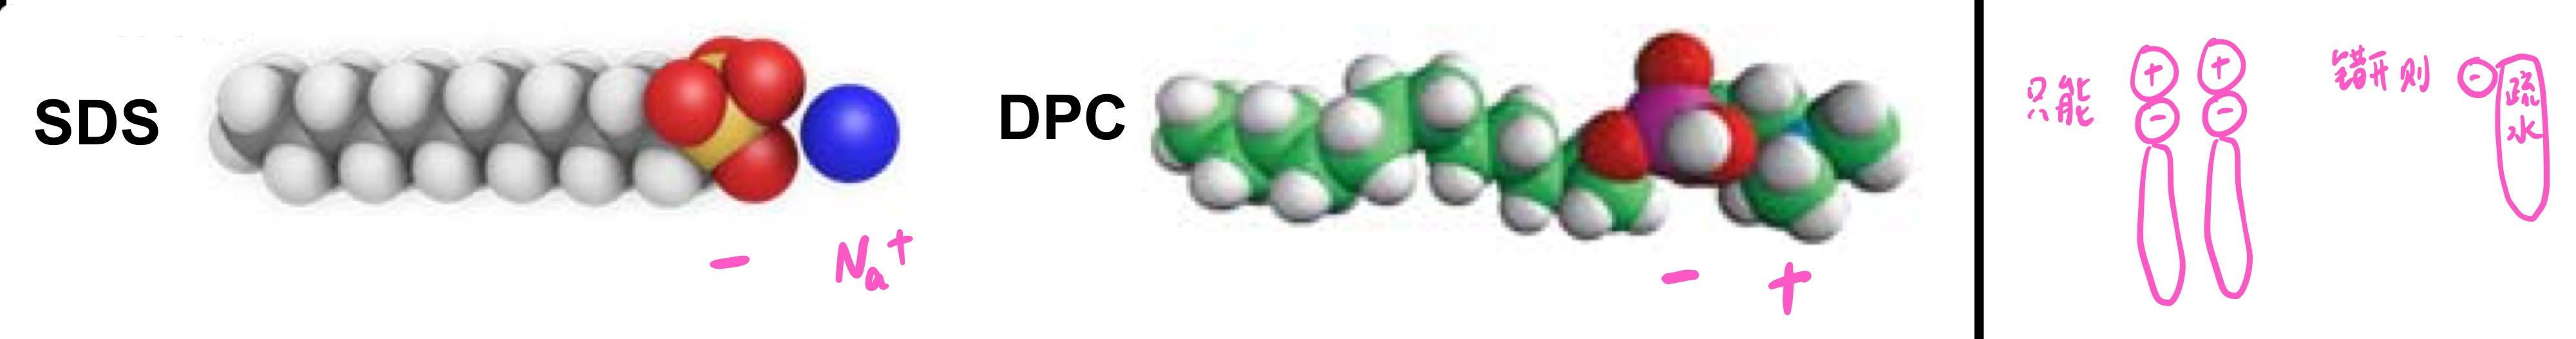
\includegraphics{3_6.jpg}
	\caption{}
\end{figure}

structure of molecules

\begin{figure}
	\centering
	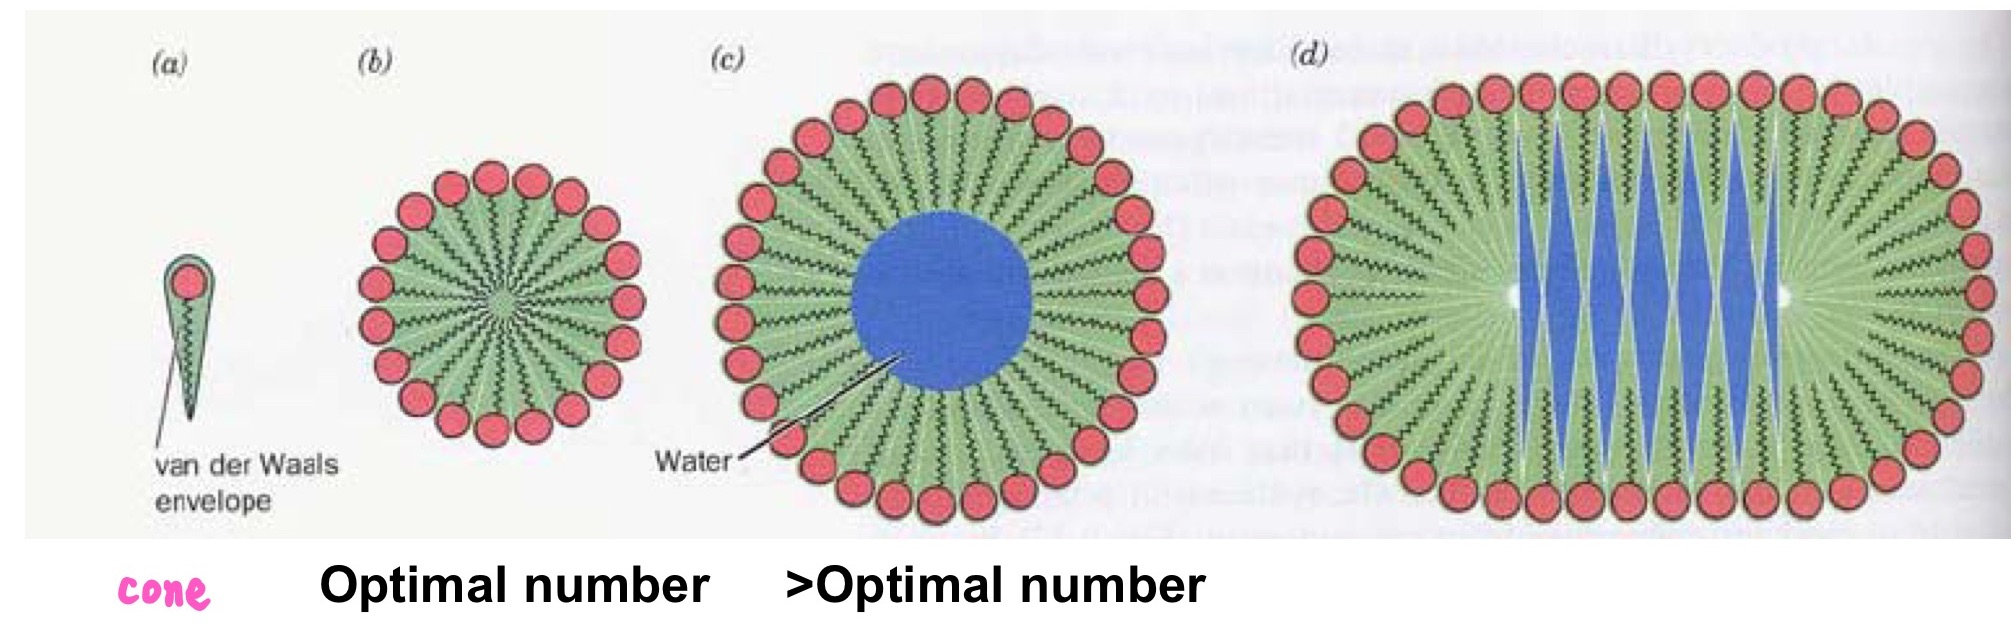
\includegraphics{3_7.jpg}
	\caption{}
\end{figure}

structure of SDS micelles

\hypertarget{lipid-mobility}{%
	\section{lipid mobility}\label{lipid-mobility}}

\begin{itemize}
	\item
	the more lipids are ordered/the closer lipids are placed, fluidity
	\(\downarrow\), melting point \(\uparrow\)
	\item
	Bilayer has two phases. gel phase: solid; fluid phase: liquid.
	\item
	saturated FAs adopt all-trans to achieve the closest contact, but all
	bonds are freely rotatable, especially those which are near the center
	of bilayer.
	
	\begin{itemize}
		\item
		gauche-\/-trans-\/-gauche makes a kink
		\item
		cis-double bond makes a bend
	\end{itemize}
	
	which reduces the packing density
	
	\begin{figure}
		\centering
		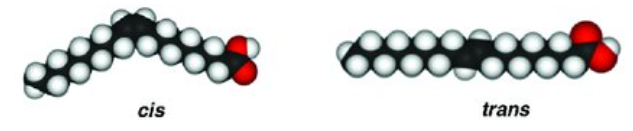
\includegraphics{3_8.png}
		\caption{}
	\end{figure}
	\item
	cholesterol
	
	\begin{itemize}
		\item
		block motions
		\item
		disrupt ordered structure
	\end{itemize}
	
	which makes a \underline{balance}, modulating the fluidity.
	
	\begin{figure}
		\centering
		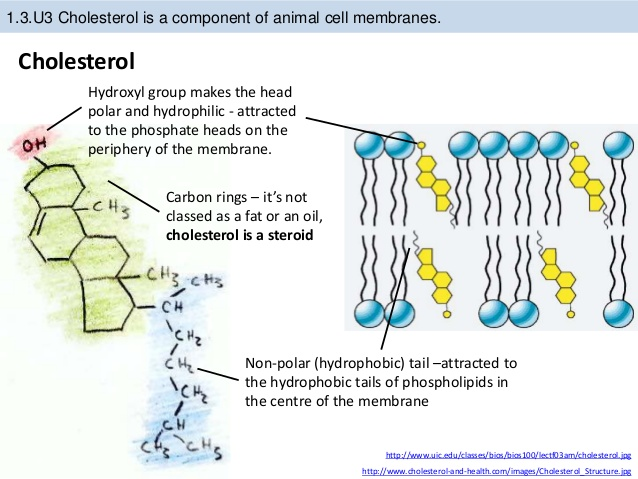
\includegraphics{3_9.jpg}
		\caption{}
	\end{figure}
	
	High conc cholesterol may abolish phase transition, keeping the
	membrane of eg. heart cells in cold blood animals functioning at a low
	tempearture.
	\item
	other motions
	
	\begin{itemize}
		\item
		lateral (侧向): much faster in fluid phase
		\item
		flip-flop: very slow
	\end{itemize}
\end{itemize}

